\documentclass[a0paper,fleqn]{betterposter/betterposter}
\usepackage{pythonhighlight}
\usepackage[
    type={CC},
    modifier={by},
    version={3.0},
]{doclicense}
\lstset{
language = Python,
backgroundcolor={\color[gray]{.95}},
breaklines = true,
basicstyle=\fontsize{30}{32}\selectfont\ttfamily,
commentstyle = {\itshape \color[cmyk]{1,0.4,1,0}},
keywordstyle = {\bfseries \color[cmyk]{0,1,0,0}},
stringstyle = {\ttfamily \color[rgb]{1,0,0}},
}

\begin{document}	
\betterposter{

\maincolumn{

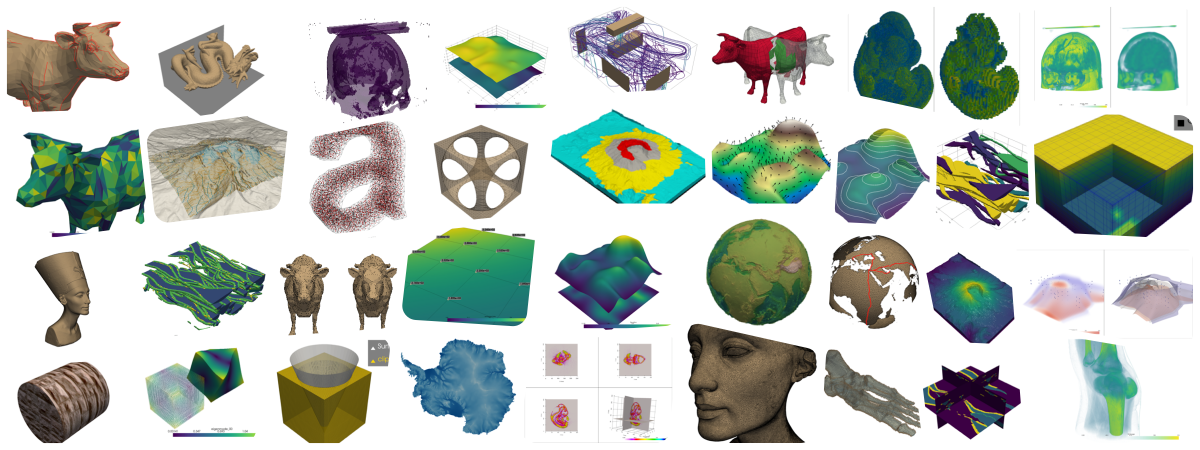
\includegraphics[width=\textwidth]{img/pyvista_banner_small}
\\ Let's plot 3D \textbf{Pythonic} visualization
\\ \$ pip install pyvista
}{

\qrcode{img/qrcode}{img/smartphoneWhite}{
\textbf{Take a picture} to
\\start tutorial
}
% Smartphone icon
% Author: Freepik
% Retrieved from: https://www.flaticon.com/free-icon/smartphone_65680

}

}{


\includegraphics[width=\textwidth]{img/logo}\\

\lstinputlisting[firstline=1, lastline=7]{hello-world.py}

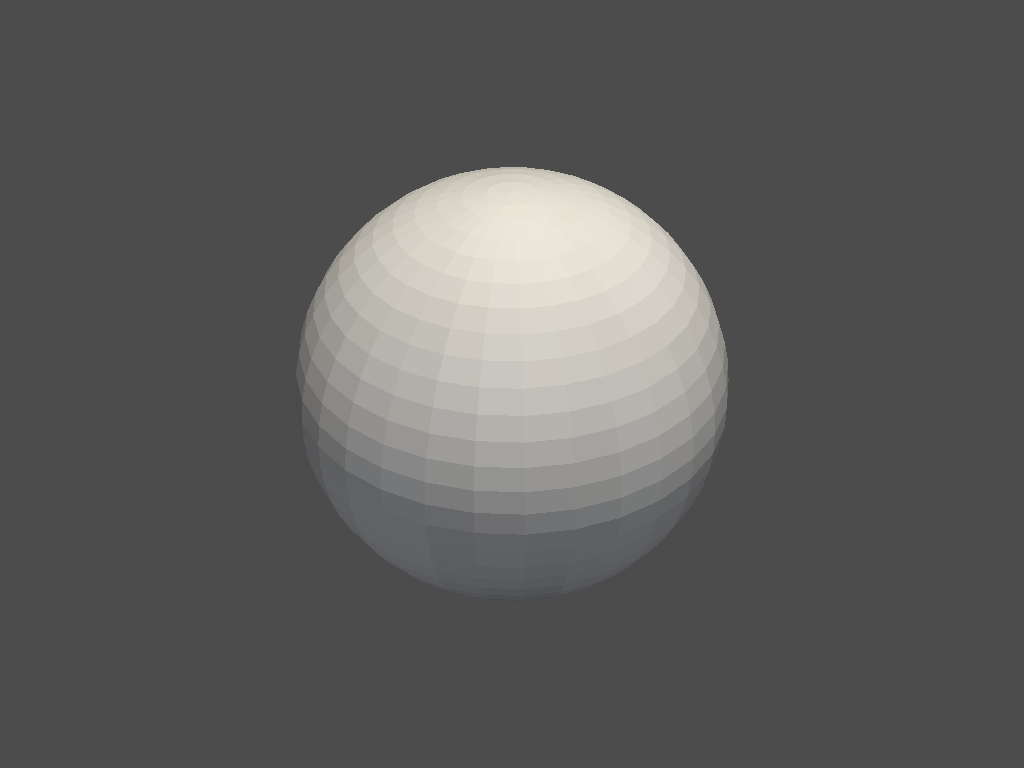
\includegraphics[width=\textwidth]{img/hello-world}

\lstinputlisting[firstline=42, lastline=48]{hello-world.py}

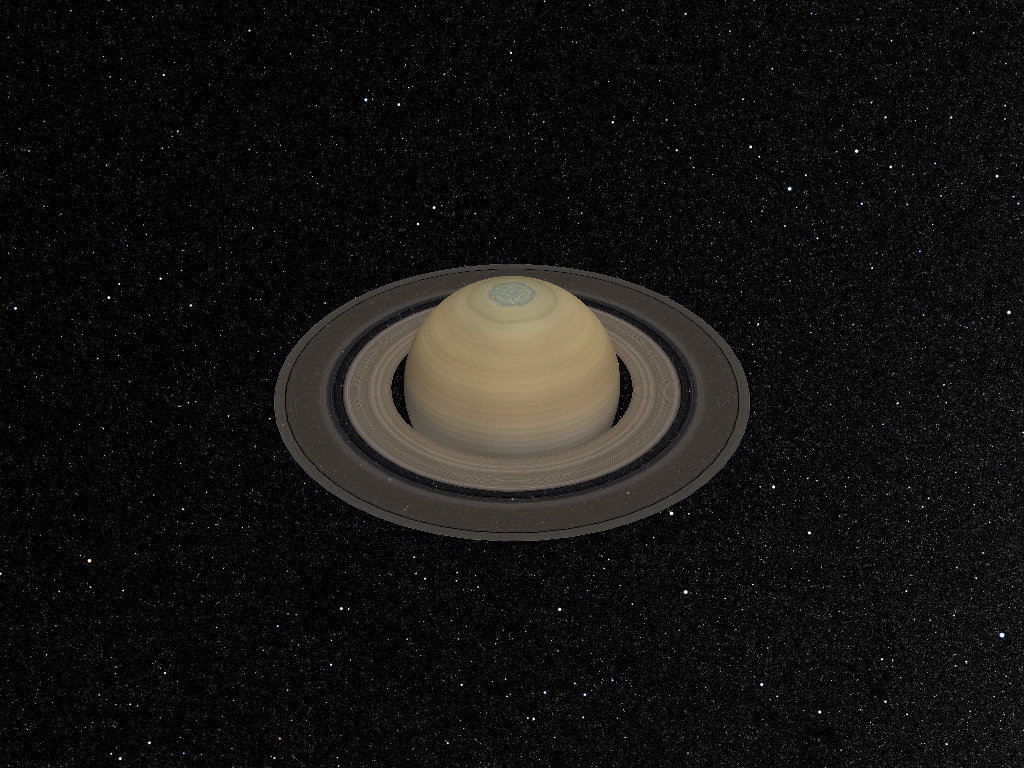
\includegraphics[width=\textwidth]{img/saturn}

\lstinputlisting[firstline=59, lastline=66]{hello-world.py}

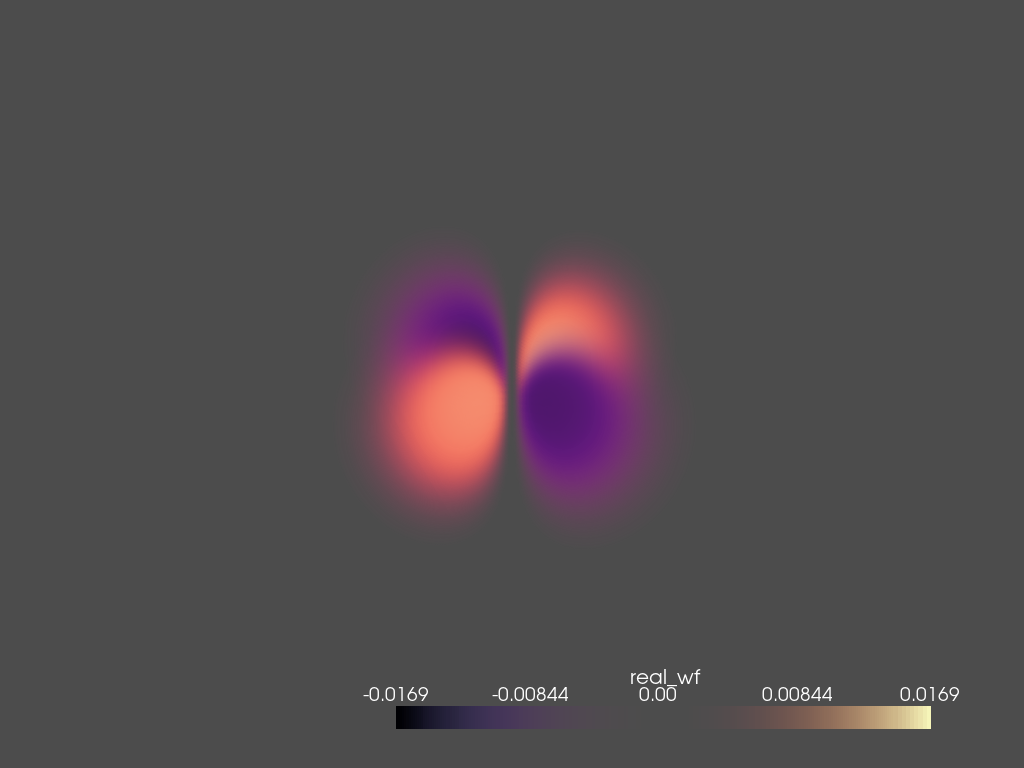
\includegraphics[width=\textwidth]{img/atom}

}{
\section{PyVista Ecosystem}


\includegraphics[width=\textwidth]{img/logo-big}\\

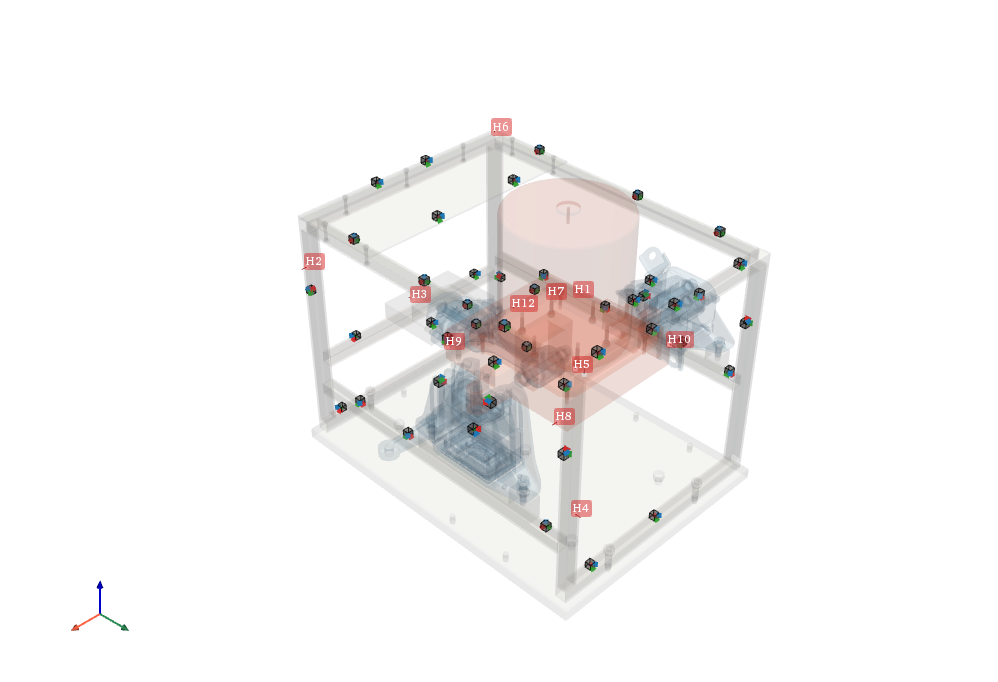
\includegraphics[width=\textwidth]{img/six_one}\\


\includegraphics[width=\textwidth]{img/geovistalogo}\\

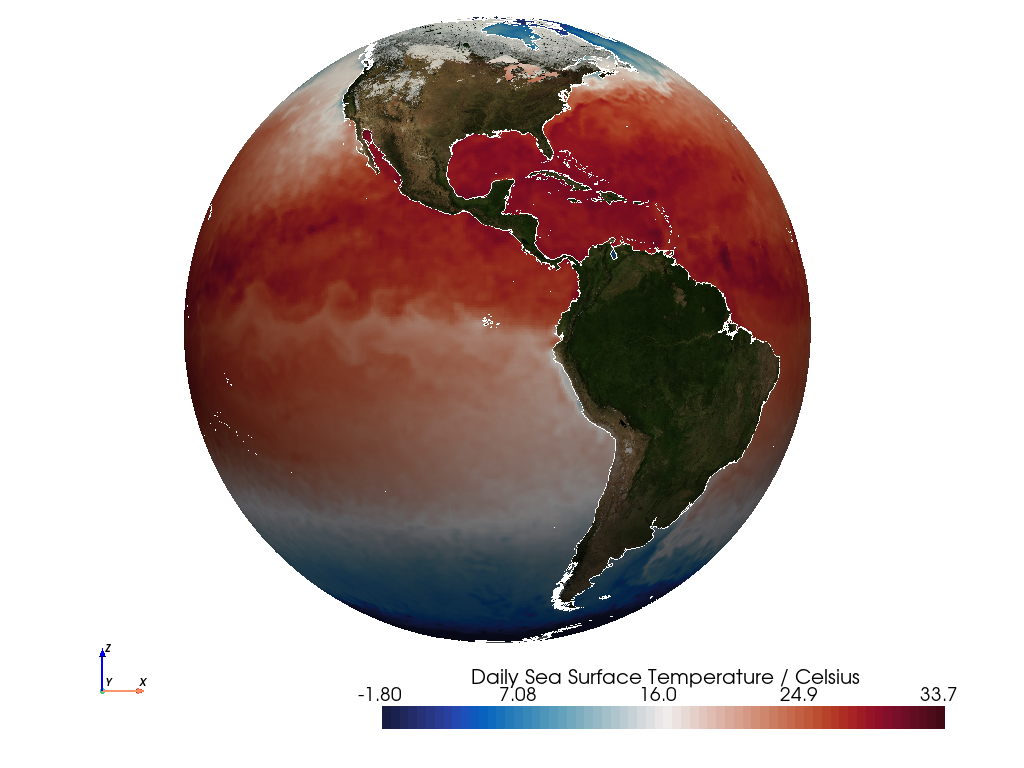
\includegraphics[width=\textwidth]{img/oisst-avhrr}\\

\doclicenseLongText\\

\begin{center}
\doclicenseImage\\
\author{PyVista Project}
\end{center}

}
\end{document}
